\section{Funzioni e chiusure}
La programmazione in stile funzionale introduce il concetto di funzioni di ordine superiore.
Si tratta di funzioni i cui parametri e/o il cui tipo di ritorno sono a loro volta una funzione.
Questo richiede, ad un linguaggio, la possibilità di trattare una funzione come un tipo dati qualsiasi, consentendo di memorizzarla in una variabile.


La differenza chiave non è sintattica, ma semantica I valori di tipo \verb|fn(...)| non catturano stato
○ Le chiusure e i tipi derivati possono includere uno stato catturato


La scelta del tipo di valore invocabile influenza vari aspetti: La
rappresentazione del valore, prestiti e possesso, modalità di invocazione,
possibilità di riuso

In Rust è possibile assegnare ad una variabile il puntatore ad una funzione (che avrà come tipo \mintinline{rust}|fn(T1,...,Tn)->U|) o assegnare un valore che implementa un tratto funzionale: \verb|FnOnce|, \verb|FnMut|, \verb|Fn|.

\subsection{Puntatori a funzione}
Qualunque sia la natura del dato assegnato, si utilizza la variabile che contiene il puntatore come se fosse essa stessa una funzione.
Sia il tipo di ritorno che tutti i tipi degli argomenti devono corrispondere a quanto dichiarato nella definizione della variabile (e della funzione).

\begin{minted}[breaklines]{rust}
fn f1(i: i32, d: f64) -> f64 { 
    return i as f64 * d; 
}

let ptr: fn(i32, f64) -> f64; 
ptr = f1; // assegno il puntatore 
ptr(2, 3.14); // chiamo la funzione 
\end{minted}

\begin{minted}[breaklines]{rust}
fn add(a: i32, b: i32) -> i32 { a + b }
fn multiply(a: i32, b: i32) -> i32 { a * b }
fn choose(c: bool) -> fn(i32, i32) -> i32 {
  if c { add } else { multiply }
}
fn main() {
  let f1 = choose(true);
  let f2 = choose(false);
  println!("f1 => {}", f1(2, 3)); // 5
  println!("f2 => {}", f2(2, 3)); // 6
}
\end{minted}



\begin{tcolorbox}
  \textbf{Nota:} fn(...) rappresenta codice invocabile senza stato catturato 
\end{tcolorbox}


\section{Funzioni lambda}
Una funzione lambda è una funzione anonima costituita da un blocco di codice espresso in forma letterale.
Tale forma dipende dal linguaggio di programmazione ed è oggetto delle forme più disparate:

\begin{itemize}
  \item \textbf{Javascript}, si utilizza la notazione freccia: \mintinline{js}|const f = (v) => v + 1|.
  \item \textbf{Kotlin}, si racchiude l'espressione tra parentesi graffe: \mintinline{kotlin}|val F = {v: Int -> v + 1}|.
  \item \textbf{C++}, si usa una notazione ancora più complessa: \mintinline{cpp}|auto f = [](int v) -> int { return v + 1; }|.
  \item \textbf{Rust}, si racchiudono i parametri formali tra \verb||||: \mintinline{rust}{let f = |v| {v + 1}}.
\end{itemize}

Una volta definita ed assegnata ad una variabile, una funzione lambda può essere invocata trattando la variabile come se fosse una funzione.
Ovvero facendo seguire al nome della variabile la lista degli argomenti racchiusi in parentesi tonde: ad esempio, \mintinline{rust}|f(5);|.

È possibile passare una funzione lambda come argomento di una funzione da invocare o utilizzare una funzione lambda come valore di ritorno di una funzione. La sintassi con cui si indica il tipo ritornato (una funzione che accetta certi tipi come parametri e restituisce un certo tipo di valore), a seconda dei linguaggi, può essere più o meno leggibile.

\begin{minted}[breaklines]{rust}
fn ret_fun() -> fn(i32) -> i32 { 
    return |x| {x + 1}; 
} 
\end{minted}


\section{Chiusure}
Il corpo di una funzione lambda può fare riferimento alle variabili che sono visibili nel contesto in cui è definita, acquisendone un riferimento, una copia o il possesso completo, in base al linguaggio e alla sintassi usata.
Tali variabili, che compaiono nel corpo della funzione lambda, sono dette \textit{variabili libere}.

La funzione lambda così ottenuta viene detta \textbf{chiusura} , in quanto racchiude, al proprio interno, (una copia de) i valori catturati (quelli contenuti nelle variabili libere), rendendoli disponibili quando sarà successivamente invocata.

In Rust, il compilatore trasforma una chiusura in una tupla avente tanti campi quante sono le variabili libere.
Tale tupla implementa uno dei tratti funzionali previsti dal linguaggio: \verb|FnOnce|, \verb|FnMut|, \verb|Fn|.


\begin{tcolorbox}
  \textbf{Note:} Una chiusura è simile ad una struct anonima con alcuni campi catturati
e con un'operazione di chiamata definita dal compilatore 
\end{tcolorbox}


\subsection{Cattura delle variabili}
Per default in Rust, tutte le variabili libere che compaiono nel corpo di una funzione lambda sono catturate per riferimento.
Il compilatore, automaticamente, crea un prestito in lettura (\mintinline{rust}|&|).
Se occorre modificare il contenuto delle variabili catturate, occorre dichiarare la funzione lambda come mutabile (\mintinline{rust}|let mut f = |...| {....};|): in questo caso verrà creato un prestito esclusivo (\mintinline{rust}|&mut|).

Il borrow checker, come al solito, verifica che tali riferimenti siano coerenti tra loro e con il tempo di vita dei valori cui si riferiscono.
Se occorre, è possibile indicare che la funzione lambda intende acquisire il possesso dei valori contenuti nelle variabili libere.
Lo si fa anteponendo alla definizione della funzione lambda la parola chiave \mintinline{rust}|move|:

\begin{center}
  \mintinline{rust}{let f = move |...| {...};}
\end{center}

\begin{figure}[h!]
  \centering
  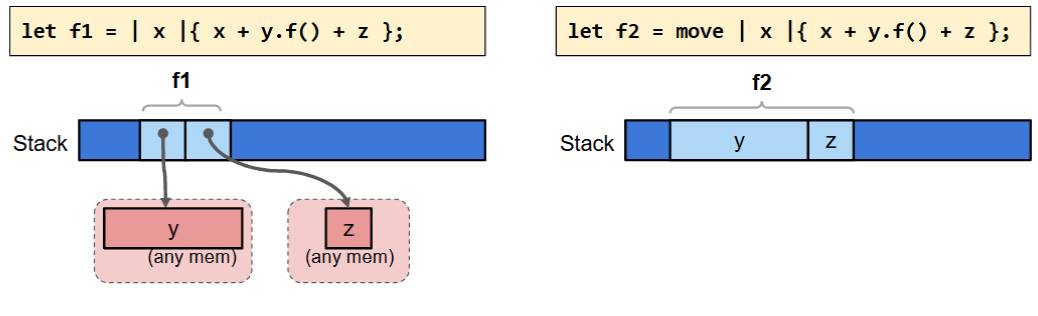
\includegraphics[width=0.6\linewidth]{content/API_Programming/images/2026-04-03-16-04-44.png}
\end{figure}


\begin{center}
  \begin{minipage}{0.75\linewidth}
    \begin{minipage}{0.48\linewidth}
      \begin{minted}[breaklines]{rust}
// Stack referenzia la memoria
let f1 = |x| { x + y.f() + z }; 
    \end{minted}
    \end{minipage}%
    \hfill
    \begin{minipage}{0.48\linewidth}
      \begin{minted}[breaklines]{rust}
// Stack possiede/copia la memoria
let f2 = move |x| { x + y.f() + z }; 
    \end{minted}
    \end{minipage}
  \end{minipage}
\end{center}


\section{I tratti funzionali}
Rust definisce tre tratti funzionali che possono essere implementati solo tramite chiusure.
Quale tratto venga implementato, dipende da cosa e come viene catturato.

\begin{minted}[breaklines]{rust}
trait FnOnce<Args> { 
    type Output; 
    fn call_once(self, args: Args) -> Self::Output; 
}

trait FnMut<Args>: FnOnce<Args> { 
    fn call_mut(&mut self, args: Args) -> Self::Output; 
}

trait Fn<Args>: FnMut<Args> { 
    fn call(&self, args: Args) -> Self::Output; 
}
\end{minted}

\subsection{Comportamento dei tratti funzionali}

\begin{itemize}
  \item \textbf{\texttt{FnOnce<Args>|}}: Una chiusura implementa questo tratto se consuma uno o più valori come parte della propria esecuzione. Pertanto, potrà essere invocata una sola volta.
  \item \textbf{\texttt{FnMut<Args>|}}: Una chiusura implementa questo tratto se può essere invocata più volte, ma ha catturato una o più variabili in modo esclusivo (\mintinline{rust}|&mut|). Questo tipo di chiusura produce effetti collaterali ed ha pertanto uno stato. Esecuzioni successive con gli stessi parametri in ingresso possono dare risultati differenti.
  \item \textbf{\texttt{Fn<Args>|}}: Una chiusura implementa questo tratto se si limita ad accedere in sola lettura alle variabili libere (\mintinline{rust}|&|). Finché la funzione esiste, le variabili libere sono in prestito condiviso e non possono essere cambiate. Pertanto, la chiusura può essere invocata un numero qualsiasi di volte e produce, a parità di argomenti, sempre lo stesso risultato.
\end{itemize}


\begin{center}
  \begin{minipage}{0.48\linewidth}
    \begin{tcolorbox}[title=Esempio FnOnce]
      \begin{minted}[breaklines]{rust}
let range = 1..10; 
let f = || range.count(); 
let n1 = f(); // 10 
let n2 = f(); // Errore di compilazione: l'intervallo è stato consumato 
        \end{minted}
    \end{tcolorbox}
  \end{minipage}%
  \hfill
  \begin{minipage}{0.48\linewidth}
    \begin{tcolorbox}[title=Esempio FnMut]
      \begin{minted}[breaklines]{rust}
let mut sum = 0; 
let mut f = |x| sum += x; 
f(5); // ok, sum: 5 
f(7); // ok, sum: 12 
        \end{minted}
    \end{tcolorbox}
  \end{minipage}
\end{center}

\begin{tcolorbox}[title=Esempio Fn]
  \begin{minted}[breaklines]{rust}
let s = "hello"; 
let f = |v| v < s; 
f("world"); // false 
f("bye"); // true 
    \end{minted}
\end{tcolorbox}


\section{Funzioni di ordine superiore}
È possibile implementare una funzione che accetta come parametro una funzione lambda ricorrendo alla programmazione generica.
Ogni funzione lambda forma infatti un tipo a sé, la cui unica istanza è la funzione lambda stessa. Tuttavia, esse implementano tutte almeno uno dei tratti funzionali: è quindi possibile definire una funzione generica che accetta come parametro di ingresso un'istanza del tipo F, soggetta al vincolo che tale tipo deve implementare uno dei tratti funzionali.

Quale specifico tratto richiedere dipende dalla natura del codice che si intende scrivere:
\begin{itemize}
  \item \verb|FnOnce(Args)| accetterà qualsiasi chiusura, ma questa potrà essere invocata una sola volta.
  \item \verb|FnMut(Args)| e \verb|Fn(Args)| sono via via più restrittivi sulle operazioni che è lecito eseguire all'interno della funzione e più ampi nell'uso della funzione di ordine superiore.
\end{itemize}

\subsection{Restituire chiusure}
Analogamente, è possibile scrivere una funzione che restituisce una chiusura.
Se la chiusura ritornata cattura qualche variabile, occorre fare attenzione al fatto che, normalmente, ciò implica memorizzare un riferimento all'interno della chiusura stessa. Questo fatto potrebbe imporre restrizioni sul tempo di vita del dato catturato non facilmente compatibili con il fatto che la chiusura ritornata deve sopravvivere alla funzione stessa (e quindi a tutte le sue variabili locali e ai suoi argomenti).

In questa situazione, si usa comunemente il modificatore \mintinline{rust}|move| per trasferire il possesso di tali dati alla chiusura stessa.
Può, inoltre, essere necessario richiedere che il dato catturato sia clonabile, se l'esecuzione della chiusura ritornata tendesse a consumare il dato e non si volesse ridurla ad \verb|FnOnce<Args>|.

\begin{minted}[breaklines]{rust}
fn value_source<T>(v: T) -> impl Fn() -> T where T: Clone { 
    return move || { v.clone() }; 
} 
\end{minted}

\begin{tcolorbox}
  \textbf{Note:} \textbf{move} serve spesso a rendere la chiusura restituita autosufficiente
\end{tcolorbox}


\subsection{Esempio di generatore}
\begin{minted}[breaklines]{rust}
fn generator(prefix: &str) -> impl FnMut() -> String { 
    let mut i = 0; 
    let b = prefix.to_string(); 
    return move || { i += 1; format!("{}{}", b, i) } 
} 

fn main() {                                     // Output atteso:
    let mut f = generator("id_");               // id_1
    for _ in 1..5 {                             // id_2
        println!("{}", f());                    // id_3
    }                                           // id_4
} 
\end{minted}
